 \chapter{Funções logarítmicas}

O princípio básico na resolução de equações e inequações exponenciais foi a comparação de potências com mesma base. Esse princípio, no entanto, é inadequado para resolver uma equação exponencial do tipo: $10^x=2$. Na resolução dessa equação, a dificuldade está em escrever o número 2 sob a forma de potência com base 10. Com estudos feitos até aqui, não sabemos qual é o valor de $x$ nem como determiná-lo. Para solucionar este e outros problemas, vamos estudar os logaritmos.

\begin{obs}
    Dados $a$ e $b$ números reais positivos, com $a\neq 1$, chama-se logaritmo de $b$ na base $a$ o expoente $x$ ao qual se deve elevar a base $a$ de modo que a potência a $x$ seja igual a $b$. Denotamos
    \begin{equation*}
        \log_a b =x \ \ \Leftrightarrow \ \ a^x=b.
    \end{equation*}

    O valor $a$ é denominado base do logarítmo, $b$ é o logaritmando e $x$ o logaritmo.
\end{obs}

\begin{exem}
    \begin{itemize}
        \item $\log_2 8=3$ pois $2^3=8$;
        \item $\log_7 7=1$ pois $7^1=7$;
        \item $\log_2 \sqrt{2}=\frac{1}{2}$ pois $2^{\frac{1}{2}}=\sqrt{2}$;
        \item $\log_{\sqrt[2]{9}} 3=\frac{3}{2}$. De fato, $(\sqrt[3]{9})^x=3 \ \Rightarrow \ 3^{\frac{2x}{3}}=3 \ \Rightarrow \ x = \frac{3}{2}.$
    \end{itemize}
\end{exem}

Vejamos algumas propriedades importantes dos logaritmos:

\begin{prop}
    Sejam $a, b \in \R_{+}^{*} \setminus \{1\}$, e $k$ uma constante real qualquer. Se $x, y \in \R_{+}^{*}$, então:

  \begin{enumerate}
  \item $\log_{a}(a)= 1$;
  \item $\log_{a}(1)= 0$;
   \item $\log_{a}(x \cdot y)=\log_{a}(x) + \log_{a}(y)$;
   \item $\log_{a} \left(\frac{x}{y}\right)=\log_{a}(x) - \log_{a}(y)$;
   \item $\log_{a}(x^{k})= k \log_{a}(x)$;
   \item $\log_{a}(a^n)= n$;
   \item \textit{(Mudança de base)} $\log_{a}(x)=\dfrac{\log_{b}(x)}{\log_{b}(a)}$;
   \item Se $0 < a < 1$ e $x < y$, então $\log_{a}(x) > \log_{a}(y)$;
   \item Se $a> 1$ e $x < y$, então $\log_{a}(x) < \log_{a}(y)$.
  \end{enumerate}
  \end{prop}
\begin{proof}
  Vamos agora demonstrar algumas destas propriedades.

  \textbf{Propriedade 1:} $\log_{a}(a)= 1$, note que:
\begin{equation*}
\log_{a}(a)= y \Leftrightarrow a^y = a \Leftrightarrow a^y= a^1 \Leftrightarrow y=1
\end{equation*}

  \textbf{Propriedade 2:} $\log_{a}(1)= 0$, note que:
\begin{equation*}
\log_{a}(1)= y \Leftrightarrow a^y= 1 \Leftrightarrow a^y= a^0 \Leftrightarrow y=0
\end{equation*}

  \textbf{Propriedade 3:} $\log_{a}(x \cdot y)=\log_{a}(x) + \log_{a}(y)$, para tal definimos:
  \begin{eqnarray*}
   a^b= x & \Leftrightarrow & b= \log_{a}(x) \\
   a^c= y & \Leftrightarrow & c= \log_{a}(y) \\
   a^{b+c}= z & \Leftrightarrow & b+c= \log_{a}(z)
  \end{eqnarray*}
  com isso obtemos que
\begin{equation*}
x \cdot y= a^b \cdot a^c= a^{b+c}= z
\end{equation*}
  portanto,
\begin{equation*}
b+c= \log_{a}(z) \Rightarrow \log_{a}(x) + \log_{a}(y)= \log_{a}(x \cdot y)
\end{equation*}

  \textbf{Propriedade 4:} $\log_{a} \left(\frac{x}{y}\right)=\log_{a}(x) - \log_{a}(y)$, para tal definimos:
  \begin{eqnarray*}
   a^b= x & \Leftrightarrow & b= \log_{a}(x) \\
   a^c= y & \Leftrightarrow & c= \log_{a}(y) \\
   a^{b-c}= z & \Leftrightarrow & b-c= \log_{a}(z)
  \end{eqnarray*}
  com isso obtemos que
\begin{equation*}
\dfrac{x}{y}= \dfrac{a^b}{a^c}= a^{b-c}= z
\end{equation*}
  portanto,
\begin{equation*}
b-c= \log_{a}(z) \Rightarrow \log_{a}(x) - \log_{a}(y)= \log_{a}\left(\frac{x}{y}\right)
\end{equation*}

  \textbf{Propriedade 5:} $\log_{a}(x^k)= k \log_{a}(x)$, note que,
\begin{equation*}
\log_{a}(x^k)= \log_{a}\underbrace{(x \cdot x \cdots x)}_{k-vezes}= \underbrace{log_{a}(x) + log_{a}(x)+ \cdots + log_{a}(x)}_{k-vezes}= k \cdot log_{a}(x)
\end{equation*}

  \textbf{Propriedade 6:} $\log_{a}(a^n)= n$, note que:
\begin{equation*}
\log_{a}(a^n)= n \cdot \log_{a}(a)= n \cdot 1 = n\qedhere
\end{equation*}
\end{proof}

\section{Função logarítmica}

\begin{obs}
 Funções logarítimicas são funções $f: \mathbb{R_{+}^{*}} \rightarrow \mathbb{R} $ tais que:
\begin{equation*}
f(x) = \log_{a}(x)
\end{equation*}
 onde é dado $a \in \mathbb{R}$ satisfazendo $a>0$ e $a \neq 1$. Estas funções são denominadas funções logarítmicas de base $a$.
\end{obs}


 Observemos que dado um número real $a> 0$ e $a \neq 1$, para cada $y>0$ existe um único número real $x$ tal que $a^x= y$, já que como visto anteriormente a função exponencial $f(x)= a^x$ é bijetiva. Podemos assim definir o logaritmo de $y$ na base $a$ como sendo o número real $x$ tal que $a^x= y$. Simbolicamente,
 \destaque{\log_a(y)= x  \Leftrightarrow a^x= y}.

 Portanto, as funções logarítmica e exponencial são inversas uma da outra.

 \begin{exem} \label{ex:log-2}
  Considere a função $f: \mathbb{R_{+}^{*}} \rightarrow \mathbb{R} $ tais que:
\begin{equation*}
f(x) = \log_{2}(x) \ .
\end{equation*}
 Vamos encontrar alguns pontos do gráfico da função $f$.

  \begin{table}[H]
 \centering
 \begin{tabular}{|c|c|c|c|} \hline
 \rowcolor{gray}
 $x$ & $f(x) = \log_{2}(x)$ & $y$ \\ \hline
  $\dfrac{1}{4}$ & $f\left(\dfrac{1}{4}\right)= \log_{2}\left(\dfrac{1}{4}\right)$ & $-2$ \\ \hline
 $\dfrac{1}{2}$ & $f\left(\dfrac{1}{2}\right)= \log_{2}\left(\dfrac{1}{2}\right)$ & $-1$ \\ \hline
 $1$ & $f(1)= \log_{2}(1)$ & $0$ \\ \hline
 $2$ & $f(2)= \log_{2}(2)$ & $1$ \\ \hline
 $4$ & $f(4)= \log_{2}(4)$ & $2$ \\ \hline
 \end{tabular}
 \end{table}

% \begin{equation*}
% \log_{2}\left(\dfrac{1}{8}\right)= y \Leftrightarrow 2^y= \dfrac{1}{8} \Leftrightarrow 2^y= 2^{-3} \Leftrightarrow y=-3
% \end{equation*}
% \begin{equation*}
% \log_{2}\left(\dfrac{1}{4}\right)= y \Leftrightarrow 2^y= \dfrac{1}{4} \Leftrightarrow 2^y= 2^{-2} \Leftrightarrow y=-2
% \end{equation*}
% \begin{equation*}
% \log_{2}\left(\dfrac{1}{2}\right)= y \Leftrightarrow 2^y= \dfrac{1}{2} \Leftrightarrow 2^y= 2^{-1} \Leftrightarrow y=-1
% \end{equation*}
% \begin{equation*}
% \log_{2}(1)= y \Leftrightarrow 2^y= 1 \Leftrightarrow 2^y= 2^0 \Leftrightarrow y=0
% \end{equation*}
% \begin{equation*}
% \log_{2}(2)= y \Leftrightarrow 2^y= 2 \Leftrightarrow 2^y= 2^1 \Leftrightarrow y=1
% \end{equation*}
% \begin{equation*}
% \log_{2}(4)= y \Leftrightarrow 2^y= 4 \Leftrightarrow 2^y= 2^2 \Leftrightarrow y=2
% \end{equation*}
% \begin{equation*}
% \log_{2}(8)= y \Leftrightarrow 2^y= 8 \Leftrightarrow 2^y= 2^3 \Leftrightarrow y=3
% \end{equation*}

   \begin{center}
    \begin{tikzpicture}[scale=1]
    \tkzInit[xmin=0, xmax=5, ymin=-2.5,ymax=2.5]
        %\tkzDrawXY
        \tkzAxeXY[fill=black!5]
        
        \tkzFct[thick,red,samples=40,domain=0.01:5]{log(x)/0.693}
        \tkzDrawPoint[fill=red, size=3](1,0)
        \tkzDrawPoint[fill=red, size=3](2,1)
        \tkzDrawPoint[fill=red, size=3](4,2)
        \tkzDrawPoint[fill=red, size=3](0.5,-1)
        \tkzDrawPoint[fill=red, size=3](0.25,-2)

        %\draw[red, above right] (2,1) node{$f(x)$};
        %\draw[blue, above right] (1,2) node{$f^{-1}(x)$};
        %\tkzDefPointByFct[ref=A, with=a](-1)
        %\tkzDefPoint(0,4){A}
        %\tkzDefPoint(2,0){B}
        %\tkzPointShowCoord(A)
        %\tkzDrawPoint[fill=red, size=3](A)
        %\tkzDrawPoint[fill=red, size=3](B)
    \end{tikzpicture}
    \end{center}
 % \begin{figure}[H]
 %    \centering
 %    \fbox{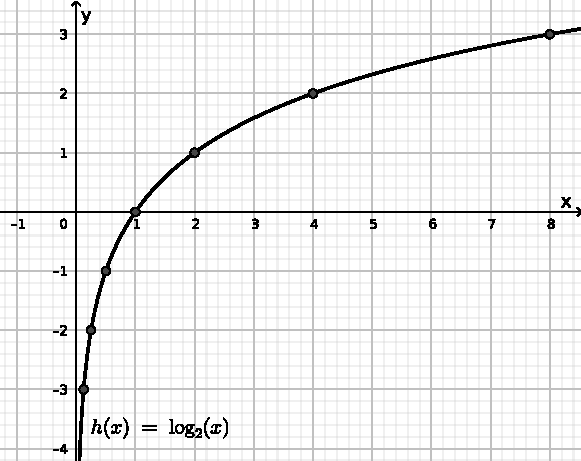
\includegraphics[width=7cm]{./cap_explog/figs/h(x)=log_2}}
 %    \caption{Gráficos da função $h(x)= \log_{2}(x)$}
 %   \end{figure}
 Observe que a função $f(x)= \log_{2}(x)$ é estritamente crescente. Veremos que sempre que $a>1$ a função $f(x)= \log_{a}(x)$ será estritamente crescente e seu gráfico será parecido com este.
 \end{exem}

 \begin{exem} \label{ex:log-1/2}
    Considere a função $f: \mathbb{R_{+}^{*}} \rightarrow \mathbb{R} $ tais que:
\begin{equation*}
f(x) = \log_{\frac{1}{2}}(x) \ .
\end{equation*}
 Vamos encontrar alguns pontos do gráfico da função $f$.

  \begin{table}[H]
 \centering
 \begin{tabular}{|c|c|c|c|} \hline
 \rowcolor{gray}
 $x$ & $f(x) = \log_{\frac{1}{2}}(x)$ & $y$ \\ \hline
  $\dfrac{1}{4}$ & $f\left(\dfrac{1}{4}\right)= \log_{\frac{1}{2}}\left(\dfrac{1}{4}\right)$ & $2$ \\ \hline
 $\dfrac{1}{2}$ & $f\left(\dfrac{1}{2}\right)= \log_{\frac{1}{2}}\left(\dfrac{1}{2}\right)$ & $1$ \\ \hline
 $1$ & $f(1)= \log_{\frac{1}{2}}(1)$ & $0$ \\ \hline
 $2$ & $f(2)= \log_{\frac{1}{2}}(2)$ & $-1$ \\ \hline
 $4$ & $f(4)= \log_{\frac{1}{2}}(4)$ & $-2$ \\ \hline
 \end{tabular}
 \end{table}

% \begin{equation*}
% \log_{\frac{1}{2}}\left(\dfrac{1}{8}\right)= y \Leftrightarrow \left(\dfrac{1}{2}\right)^y= \dfrac{1}{8} \Leftrightarrow \left(\dfrac{1}{2}\right)^y= \left(\dfrac{1}{2}\right)^{3} \Leftrightarrow y=3
% \end{equation*}

   \begin{center}
    \begin{tikzpicture}[scale=1]
    \tkzInit[xmin=0, xmax=5, ymin=-2.5,ymax=2.5]
        %\tkzDrawXY
        \tkzAxeXY[fill=black!5]
        
        \tkzFct[thick,red,samples=40,domain=0.01:5]{-log(x)/0.693}
        \tkzDrawPoint[fill=red, size=3](1,0)
        \tkzDrawPoint[fill=red, size=3](2,-1)
        \tkzDrawPoint[fill=red, size=3](4,-2)
        \tkzDrawPoint[fill=red, size=3](0.5,1)
        \tkzDrawPoint[fill=red, size=3](0.25,2)

        %\draw[red, above right] (2,1) node{$f(x)$};
        %\draw[blue, above right] (1,2) node{$f^{-1}(x)$};
        %\tkzDefPointByFct[ref=A, with=a](-1)
        %\tkzDefPoint(0,4){A}
        %\tkzDefPoint(2,0){B}
        %\tkzPointShowCoord(A)
        %\tkzDrawPoint[fill=red, size=3](A)
        %\tkzDrawPoint[fill=red, size=3](B)
    \end{tikzpicture}
    \end{center}
    
 % \begin{figure}[H]
 %    \centering
 %    \fbox{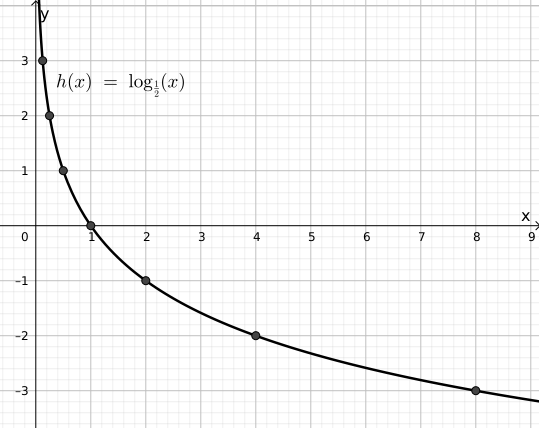
\includegraphics[width=7cm]{./cap_explog/figs/h(x)=log_12}}
 %    \caption{Gráficos da função $h(x)= \log_{1/2}(x)$}
 %   \end{figure}
 Observe que a função $f(x)= \log_{1/2}(x)$ é estritamente decrescente. Veremos que sempre que $0< a< 1$ a função $f(x)= \log_{a}(x)$ será decrescente e seu gráfico será parecido com este.
 \end{exem}

 Para facilitar a comparação dos gráficos das funções dos dois últimos exemplos observe o plano cartesiano abaixo no qual temos os dois gráficos, note que eles são simétricos em relação ao eixo $x$.

 %   \begin{figure}[H]
 % \centering
 %    \fbox{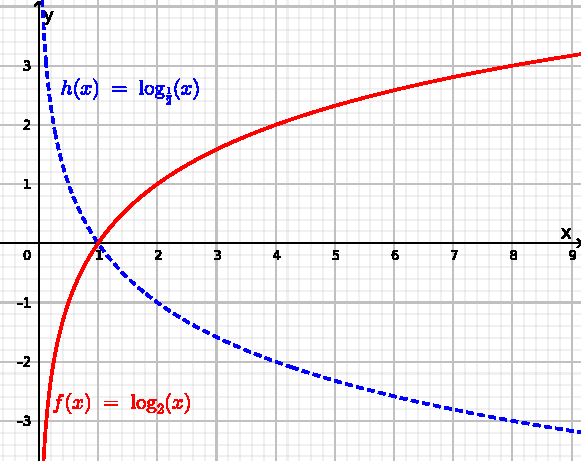
\includegraphics[width=8cm]{./cap_explog/figs/comparandologs}}
 %    %\caption{Comparando gráficos de funções logarítmicas}
 %  \end{figure}


  \begin{exem} \label{ex:log-e}
   Um caso especial de função logarítmica é quando $a= e$, assim $f: \mathbb{R_{+}^{*}} \rightarrow \mathbb{R} $ será dada por:
\begin{equation*}
f(x) = \log_{e}(x)= \ln(x)
\end{equation*}
  esta função é chamada logaritmo natural, que é uma função crescente, e seu gráfico é:

   \begin{center}
    \begin{tikzpicture}[scale=1]
    \tkzInit[xmin=0, xmax=5, ymin=-2.5,ymax=2.5]
        %\tkzDrawXY
        \tkzAxeXY[fill=black!5]
        
        \tkzFct[thick,red,samples=50,domain=0.1:5]{log(x)}
        % \tkzDrawPoint[fill=red, size=3](1,0)
        % \tkzDrawPoint[fill=red, size=3](2,1)
        % \tkzDrawPoint[fill=red, size=3](4,2)
        % \tkzDrawPoint[fill=red, size=3](0.5,-1)
        % \tkzDrawPoint[fill=red, size=3](0.25,-2)

        %\draw[red, above right] (2,1) node{$f(x)$};
        %\draw[blue, above right] (1,2) node{$f^{-1}(x)$};
        %\tkzDefPointByFct[ref=A, with=a](-1)
        %\tkzDefPoint(0,4){A}
        %\tkzDefPoint(2,0){B}
        %\tkzPointShowCoord(A)
        %\tkzDrawPoint[fill=red, size=3](A)
        %\tkzDrawPoint[fill=red, size=3](B)
    \end{tikzpicture}
    \end{center}

 \end{exem}

  Anteriormente comentamos que a função exponencial de base $a$ tem como inversa a função logaritmo de base $a$, vamos agora retomar os exemplos que fizemos acima, para comparar os gráficos das exponenciais com seus respectivos logaritmos inversos. Vamos com isso observar que em todos os casos os gráficos são simétricos em relação ao gráfico da função identidade $Id(x)= x$.

  \begin{enumerate}
   \item Caso $a>1$: considere as funções $f(x)= a^x$ e $g(x)= \log_{a}(x)$ respectivamente, cujos gráficos são simétricos em relação ao gráfico da função $Id$, como pode ser visto na figura abaixo, isso ocorre pois as funções $f$ e $g$ são inversas uma da outra.

   \begin{center}
    \begin{tikzpicture}[scale=.8]
    \tkzInit[xmin=-2.5, xmax=5, ymin=-2.5,ymax=5]
        \tkzDrawXY[noticks]
        %\tkzAxeXY%[fill=black!5]
        
        \tkzFct[thick,red,samples=50,domain=0.1:5]{log(x)/0.693}
        \tkzFct[thick,blue,samples=40,domain=-2.5:2.5]{2**x}
        \tkzFct[thick,gray,samples=2,domain=-1.5:4.5]{x}
        % \tkzDrawPoint[fill=red, size=3](1,0)
        % \tkzDrawPoint[fill=red, size=3](2,1)
        % \tkzDrawPoint[fill=red, size=3](4,2)
        % \tkzDrawPoint[fill=red, size=3](0.5,-1)
        % \tkzDrawPoint[fill=red, size=3](0.25,-2)

        \draw[red, below right] (2,1) node{$g(x)=log_a(x)$};
        \draw[blue, above left] (1,2) node{$f(x)=a^x$};
        %\tkzDefPointByFct[ref=A, with=a](-1)
        %\tkzDefPoint(0,4){A}
        %\tkzDefPoint(2,0){B}
        %\tkzPointShowCoord(A)
        %\tkzDrawPoint[fill=red, size=3](A)
        %\tkzDrawPoint[fill=red, size=3](B)
    \end{tikzpicture}
    \end{center}
    
   % \begin{figure}[H]
   %  \centering
   %  \fbox{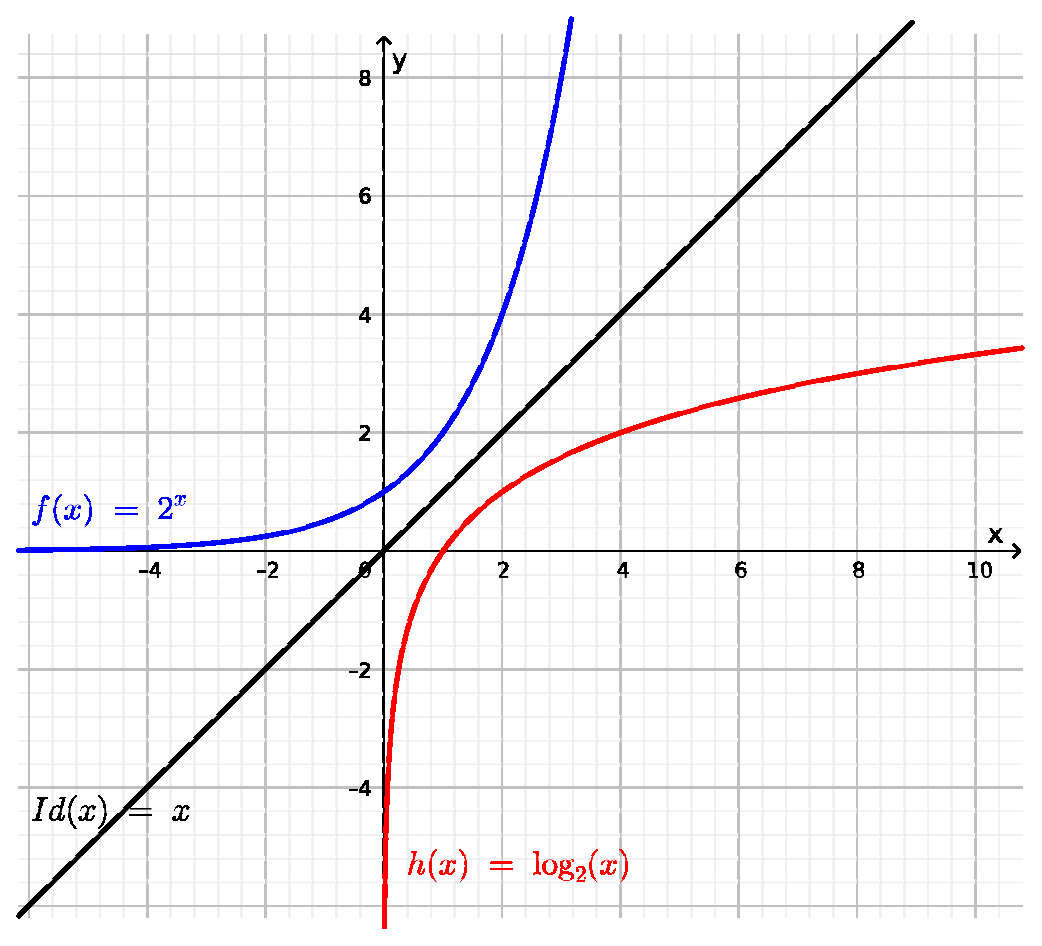
\includegraphics[width=9cm]{./cap_explog/figs/comparandobase2}}
   %  \caption{Gráficos das funções exp e log de base $2$}
   % \end{figure}

   \item Caso $0<a<1$: considere as funções $f(x)= a^x$ e $g(x)= \log_a(x)$ respectivamente, cujos gráficos são simétricos em relação ao gráfico da função $Id$, como pode ser visto na figura abaixo, isso ocorre pois as funções $f$ e $g$ são inversas uma da outra.

   \begin{center}
    \begin{tikzpicture}[scale=0.8]
    \tkzInit[xmin=-2.5, xmax=5, ymin=-2.5,ymax=5]
        \tkzDrawXY[noticks]
        %\tkzAxeXY%[fill=black!5]
        
        \tkzFct[thick,red,samples=80,domain=0.01:5]{-log(x)/0.693}
        \tkzFct[thick,blue,samples=60,domain=-2.5:5]{2**(-x)}
        \tkzFct[thick,gray,samples=2,domain=-1.5:4.5]{x}
        % \tkzDrawPoint[fill=red, size=3](1,0)
        % \tkzDrawPoint[fill=red, size=3](2,1)
        % \tkzDrawPoint[fill=red, size=3](4,2)
        % \tkzDrawPoint[fill=red, size=3](0.5,-1)
        % \tkzDrawPoint[fill=red, size=3](0.25,-2)

        \draw[red, above right] (0.1,3) node{$g(x)=log_a(x)$};
        \draw[blue, above right] (3,0.1) node{$f(x)=a^x$};
        %\tkzDefPointByFct[ref=A, with=a](-1)
        %\tkzDefPoint(0,4){A}
        %\tkzDefPoint(2,0){B}
        %\tkzPointShowCoord(A)
        %\tkzDrawPoint[fill=red, size=3](A)
        %\tkzDrawPoint[fill=red, size=3](B)
    \end{tikzpicture}
    \end{center}
   % \item Considere os exemplos \ref{ex:exp-e} e \ref{ex:log-e}, nestes exemplos apresentamos as funções $f(x)= e^x$ e $h(x)= \ln(x)$ respectivamente, cujos gráficos são simétricos em relação ao gráfico da função $Id$, como pode ser visto na figura abaixo, isso ocorre pois as funções $f$ e $h$ são inversas uma da outra.

   % \begin{figure}[H]
   %  \centering
   %  \fbox{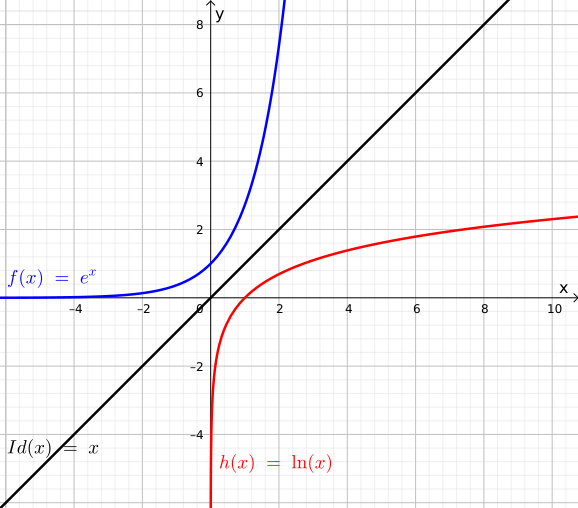
\includegraphics[width=9cm]{./cap_explog/figs/comparandobase-e}}
   %  \caption{Gráficos das funções exp e log de base $e$}
   % \end{figure}
  \end{enumerate}

\section{Equações logarítmicas}

\begin{obs}
    Equações logarítmicas são equações que envolvem logaritmos.
\end{obs}

Para resolvê-las, seguimos os passos 
seguintes:
\begin{enumerate}
    \item Encontrar restrição: estabelecemos as condições de existência, encontrando os valores de $x$ para os quais existem todos os logaritmos mencionados na equação; para isso, os logaritmandos devem ser positivos e as bases, positivas e diferentes de 1 (conforme a definição de logaritmo)
    \item Resolver a equação: Aplicamos a definição e as propriedades dos logaritmos para obter os valores de $x$ que, se satisfazerem as condições de existência, serão soluções da equação. Podemos ter duas situações a resolver:
    \begin{itemize}
        \item Se $\log_a f(x) = k $ então $ f(x)=a^k$;
        \item Se $\log_a f(x) = \log_a g(x) $ então $ f(x)=g(x)$.
    \end{itemize}
\end{enumerate}

\begin{exem}
    $\log_2 (3x+1) = 4$
    
    Veja que a solução deve satisfazer $3x+1>0$, isto é, $x>-\frac{1}{3}$. Assim,
    \begin{align*}
        \log_2 (3x+1) &= 4\\
        3x+1&=2^4\\
        x=5.
    \end{align*}
    Portanto, $S={5}$.
\end{exem}

\begin{exem}
    $\log (x+2) + \log(x-2) = \log (3x)$
    
    A solução deve satisfazer 
    \begin{equation*}
        \left\{
        \begin{matrix}
            x+2>0\\
            x-2>0\\
            3x>0
        \end{matrix}
        \right.
        \ \Rightarrow \ 
        x>2.
    \end{equation*}
    
    Assim,
    \begin{align*}
        \log (x+2) + \log(x-2) &= \log (3x)\\
        \log (x+2)(x-2) &= \log (3x)\\
        (x+2)(x-2) &= 3x\\
        x^2-4&=3x\\
        x^2-3x-4=0.
    \end{align*}

    Resolvendo a equação, obtemos as raízes $4$ e $-1$. No entanto, a solução da equação inicial deve satisfazer $x>2$. Portanto, $S={4}$.
\end{exem}

  \section{Inequações logarítmicas}
 
\begin{obs}
 As inequações logarítmicas são inequações que envolvem funções logarítmicas
\end{obs}
 
 A resolução das inequações logarítmicas se dividem em dois casos, a depender do valor da base $a$, são eles:
 
 Caso 1: $a > 1$ temos que,
  \begin{eqnarray*}
 \log_a x > \log_a y \ \Rightarrow \ x>y
 \end{eqnarray*}
 ou seja, neste caso a desigualdade se mantém.

 Caso 2: $0< a < 1$ temos que,
  \begin{eqnarray*}
 \log_a x > \log_a y \ \Rightarrow \ x<y
 \end{eqnarray*}
 ou seja, nesta situação ocorre uma inversão da desigualdade.
 
  \begin{exem}
  $\log_3(2x+1)>\log_3 7$.

  A restrição da solução é $2x_1>0$, ou seja, $x>-\frac{1}{2}$. Assim,
  \begin{align*}
      \log_3(2x+1) &>\log_3 7\\
      2x+1&>7\\
      x>3.
  \end{align*}

  A solução é a interseção de $(3,+\infty)$ com a restrição $(-\frac{1}{2},+\infty)$. Logo, $S=(3,+\infty)$.
  \end{exem}

    \begin{exem}
  $\log_{\frac{1}{2}}(2x+1)>\log_{\frac{1}{2}} 9$.

  A restrição da solução é $2x_1>0$, ou seja, $x>-\frac{1}{2}$. Assim,
  \begin{align*}
      \log_{\frac{1}{2}}(2x+1)&>\log_{\frac{1}{2}} 9\\
      2x+1&<9\\
      x<4.
  \end{align*}

  A solução é a interseção de $(-\infty,4)$ com a restrição $(-\frac{1}{2},+\infty)$. Logo, $S=(-\frac{1}{2},4)$.
  \end{exem}
\begin{secExercicios}

\begin{exer}
    Calcule:
    \begin{enumerate}[a)]
        \begin{multicols}{2}
        \item $\log_3 9$
        \item $\log_2 128$
        \item $\log 1000$
        \item $\log_8 16$
        \item $\log_{\frac{1}{4}} 32$
        \item $\log_{\sqrt[3]{7}} 49$
        \end{multicols}
    \end{enumerate}
\end{exer}

\begin{exer}
    Qual o valor da expressão
    \begin{equation*}
        \dfrac{\log_5 1 +\log_{10} 0,01}{\log_2 64 \cdot \log_4 \sqrt{8}}.
    \end{equation*}
\end{exer}

\begin{exer}
    Determine o conjunto solução das seguintes equações:
    \begin{enumerate}[a)]
        \item $\log_{11} (7x-2)=\log_{11} 5$
        \item $\log_3 \dfrac{x+3}{x-1}=1$
        \item $\log_x 243 =5$
        \item $\log_x \frac{1}{9}=2$
        \item $\log_6 x + \log_6 (x-1) = 1$
        \item $ \log_{10} x +\log_{10}(2x) = 1 $
        \item $2\log_{2}x - \log_{2}(x+\frac{5}{4})=2$
        \item $(\log_2 x)^2 - 3 \log_2 x -4=0$
        \item $\log_{\frac{1}{2}}(\log_9 2x)=1$
        \item $|1+\log_3 x|=2$
        \item $(\log_2 x)^2 - 9 \log_8 x=4$
    \end{enumerate}
\end{exer}

\begin{exer}
    Dê o maior domínio das funções:
    \begin{enumerate}[a)]
        \item $f(x)=\log_4 (x^2-6x+8)$
        \item $f(x)=\log \dfrac{x-4}{x+1}$
        \item $f(x)=\log_{x^2-4x+4} 72$
        \item $f(x)=\log_{x-3} (x^2-7x+10)$
    \end{enumerate}
\end{exer}

\begin{exer}
    Resolva as inequações:
    \begin{enumerate}[a)]
        \item $\log_3(x+6)>\log_3 11$
        \item $\log_8(4x-6)<\log_8 18$
        \item $\log_3(x+2)<2$
        \item $\log_{\frac{1}{5}}(2x-1)<-2$
        \item $\log_5(x-7)>2 \log_5 6$
    \end{enumerate}
\end{exer}

\begin{exer}
    Construa o gráfico das funções:
    \begin{enumerate}[a)]
        \item $f(x)=\log_2 (x+1)$
        \item $f(x)=\log |x|$
        \item $f(x)=\log_2 (x+1)$
    \end{enumerate}
\end{exer}

\begin{exer}
    Considere a função  real $f: A \to \R$ dada por
    \begin{align*}
    f(x) = \log\left(\frac{1}{x-1}\right)
    \end{align*}
    
    \begin{enumerate}[a)]
    \item Determine o maior domínio de $f$.
    \item Esboce o gráfico de $f$.
    \item Exiba a expressão $f^{-1}$ e esboce seu gráfico.
    \item A função $g: A\to \R_{+}$ dada por $g(x) = |f(x)|$ é inversível? Justifique.
    \end{enumerate}
\end{exer}

% \begin{exer}
%     Considere a função $f:A \to \R$ dada por $f(x) = \log_{3}(x+3)$.
%     \begin{enumerate}[a)]
%     \item Esboce o gráfico de $f$.
%     \item Determine o maior domínio real $A$ e a imagem de $f$.
%     \item A função $g: A\to \R_{+}$ dada por $g(x) = |f(x)|$ é inversível? Justifique.
%     \end{enumerate}
% \end{exer}

\begin{exer}
    (UFSCar-SP) A altura média do tronco de certa espécie de árvore evolui, desde que é plantada, segundo o seguinte modelo matemático:
    \begin{equation*}
        h(t)=1,5 +\log_3 (t+1),
    \end{equation*}
    com $h(t)$ em metros e $t$ em anos. Se uma dessas árvores foi cortada quando seu tronco atingiu 3,5m de altura, determine o tempo (em anos) transcorrido do momento da plantação até o corte.
\end{exer}

\end{secExercicios}

%\subsection*{Respostas}

%\shipoutAnswer
